%lost on page 11 - extracted and used climate variables
%Maybe reordering stuff on paragraph
%cartoon of whole procedure for climate variables
%figure showing correlation b/t bio12 and 
%state that VSURF importance is different scales in different models
%moved up three hypotheses part to introduction
%play up lack of GxE and ???
%** correct # of Pop x Treatment

%* delve into interactions - do they change cline?

%* show figures of reaction norms
%* split plot, account for error variation in temp???
%* show PAR similarity
%* what CO2 concentration did I use?
%* some sites they are functionally annual

%* hung up on specialization - clarify? where is ecological oppportunity, tradeoffs, specialization
%	- maybe temporal source-sink makes more sense

%* check out matthew's blog on hydrology variables

%* explain rhizomes

%* put in biomass allocation cline
% TO DO:
% 1. Is water regime on figure 1 correct?
% 2. Finalize Table 2
% 3. Do anything with biomass data?
% 4. Citations for latitudinal clines
	% cases where clinal variation has 'obvious' selective source:
	% Antonovics and Bradshaw discuss steepness of clines and strength of selection over 10's of meters off mines in Anthoxanthum
	% Caicedo et al 2004?
	% clines in phenotypic traits reviewed by Hedrick 2006, Schemske and Bier 2007
% 5. Citations for GxE as signature of local adaptation
% 6. Fix figure 2
% 7. Supplemental Figure and Table captions
% 8. Supplemental figure showing agreement between assigned to climatic variables from point estimated and spatially averaged analyses

\documentclass[11pt, oneside]{article}

%
% Packages
%

\usepackage{geometry}
\geometry{letterpaper}
\usepackage[parfill]{parskip}      		% Activate to begin paragraphs with an empty line rather than an indent
\usepackage{graphicx}
\usepackage{booktabs}
\usepackage{topcapt}
\usepackage[labelfont =  {sf, bf}, textfont = sf, format = plain]{caption}
\usepackage{amssymb}
\usepackage{amsmath}
\usepackage{natbib}
\usepackage{color}
\usepackage{array}
\usepackage{gensymb}
\usepackage{setspace}
\newcommand{\stretchy}{1.5}
\usepackage{lineno}
\usepackage{textcomp}

% Make helvetica the default sans-serif font
% \renewcommand\sfdefault{phv}

% Package command for citing R packages
\newcommand{\pkg}[1]{{\fontseries{b}\selectfont #1}} 

%
% Commenting
%

\newcommand{\cdm}[1]{{ \color{magenta} [{\bf{CDM:}} {\em#1}]}} % Chris' comments are in magenta.
\newcommand{\ala}[1]{{ \color{blue} [{\bf{ALA:}} {\em#1}]}} % Amy's comments are in blue.

%
% Where to find files
%


%
% Title and authors
%

\title{Grow with the flow: faster growth is associated with more variable precipitation in a perennial herb}
\author{Christopher D. Muir$^{1,*}$ and Amy L. Angert$^1$}
\date{}

%
% Start document
%

\usepackage{Sweave}
\begin{document}
\Sconcordance{concordance:ms.tex:ms.Rnw:%
1 77 1 1 47 13 1 1 0 53 1 1 10 56 1 1 113 39 1 1 18 4 1 1 46 1 1 1 47 3 %
1 1 16 3 1 1 12 11 1 1 50 1 5 9 1 1 222 255 1 1 17 51 1 1 14 51 1 1 14 %
49 1 1 15 56 1 1 11 89 1}

\maketitle

$^1$ Biodiversity Research Centre, University of British Columbia, Vancouver, BC, Canada \\
$^*$corresponding author: Chris Muir, cdmuir@biodiversity.ubc.ca \\

Original Article \\

Key words: local adaptation, cline, photosynthesis, growth rate, \textit{Mimulus} \\

Word counts: TBA \\
3 figures; 3 tables; ? supporting files \\
Data will be archived on Dryad upon acceptance. \\

\cdm{Chris' comments}\\
\ala{Amy's comments}

\clearpage

\listoffigures
\listoftables

\section*{Abstract}

Local adaptation is one of the most ubiquitous observations in nature: organisms perform well in their natal environment, but poorly outside it. Correlation between traits and latitude, or latitudinal clines, are among the most common pieces of evidence for local adaptation, but identifying the traits under selection and the selective agents are challenging. Here, we investigated a latitudinal cline in growth and photosynthesis across 16 populations of the perennial herb \textit{Mimulus cardinalis} (Phrymaceae). Using machine learning methods, we identify interannual variation in precipitation as a likely selective agent: Southern populations from more variable environments had higher photosynthetic rates and grew faster. We hypothesize that selection may favor a more annualized life history -- grow now rather than save for next year -- in environments where severe droughts occur more often. Thus our study provides insight into how species may adapt if Meditteranean climates become more variable due to climate change.

\setstretch{\stretchy}

\section*{Introduction}

% Toggle these commands to get version for doing word count
% \linenumbers
% \pagenumbering{gobble}
% \raggedright

% Local adaptation and clines
Local adaptation within species is ubiquitous; populations generally have higher fitness in their native environment, but perform poorly outside it \citep{Schluter_2000, Hereford_2009}. Local adaptation also frequently leads to clines in both phenotypes and allele frequencies when selection varies over environmental gradients \citep{Huxley_1938, Endler_1977}. Phenotypic differences between populations along a cline most often have a genetic basis and can be studied in a common garden \citep{Turesson_1922, Clausen_etal_1940, Hiesey_etal_1942}. Despite a long history of studying local adaptation and clines, it remains to challegenging to identify exactly which traits are under selection and which differ for nonadaptive reasons. In particular, the role that physiological differences play in local adaptation is poorly understood, despite the fact that physiology is frequently assumed to explain adaptation to the abiotic environment. We need to understand physiological adaptations within species as a baseline for anticipating how organisms will respond to climate change. A related problem is identifying which features of the environment, abiotic factors like soil water availability or biotic interactions, cause spatially varying selective pressures. Here, we examine physiological trait variation and possible selective agents in the perennial herb \textit{Mimulus cardinalis} Douglas ex Benth. (Phrymaceae), a model system for local adaptation studies.

% Intrinsic versus plastic variation
There are two basic approaches one can use to identify candidate traits underlying local adaptation in a common garden. First, if genetically-based trait differences between populations vary clinally with environmental differences, this may point to traits important for local adaptation. Second, genotype by environment interactions could indicate that variation in plasticity mediates local adaptation. We distinguish between these signatures of local adaptation by referring to `intrinsic' and `plastic' trait variation, respectively. There are classic cases of adaptation involving both intrinsic and plastic trait variation. For example, intrinsic differences in critical photoperiod [CITE] and developmental rate \citep{Stinchcombe_etal_2004} allow organisms to properly time their life history with the local environment. Conversely, sun and shade plants do not have intrinsically higher or lower rates of carbon assimilation, but rather, genotype by environment interactions cause sun plants to assimilate more under high light and shade plants under low light \citep{Givnish_1988}. In plants especially, we know little about the prevalance and adaptive significance of variation in fundamental physiological traits like photosynthesis and their impact on plant performance.

% Selective agents
Either instrinsic and/or plastic variation should vary clinally along environmental gradients.\ala{this is confusing given definitions above} Indeed, clines in ecologically important traits are widespread in nature \citep{Endler_1977} and often adaptive, but in most cases the selective agent is unknown. For example, in \textit{Drosophila} numerous latitudinal clines exist for traits like thermal tolerance \citep{Hoffmann_etal_2002}, body size (\cite{Coyne_Beecham_1987} and references therein), and life history \citep{Schmidt_etal_2005}. Some \textit{Drosophila} clines have evolved multiple times (\cite{Oakeshott_etal_1982, Huey_etal_2000}, see also \cite{Bradshaw_Holzapfel_2001}) or shifted in response to climate change \citep{Umina_etal_2005}, evincing climatic adaptation. Similarly, plant species exhibit latitudinal clines in traits like flowering time \citep{Stinchcombe_etal_2004}, cyanogenesis \citep{Kooyers_Olsen_2012}, and leaf morphology \citep{Hopkins_etal_2008} that likely relate to climatic variation. 

Despite the fact that latitudinal clines in particular have been studied for a long time, latitude \textit{per se} cannot be a selective agent. Latitude may be strongly correlated with one or two key climatic variables, such as temperature, precipitation, or growing degree-days, such that latitude is an effective proxy for the underlying climatic driver but nonetheless the key climatic variable(s) with stronger relationships to traits are identifiable. Alternatively, latitude may be more strongly related to traits than any single climatic variable for two possible reasons. First, latitude may be correlated with several climatic agents of selection that are individually weak, but add up to a strong latitudinal cline. Alternatively, gene flow among neighboring populations could smooth out local climatic effects, since alleles will experience selection across populations linked by migration. For example, in mountainous regions average temperature at a given latitude varies widely, but in aggregate, a Southern set of populations will experience warmer climate than a Northern one. Thus, any particular Southern population would be warm-adapted, even if it was located in cooler (e.g. high elevation) site. Because many climatic factors vary latitudinally, and which climatic factors vary latitudinally changes over the earth's surface (e.g. coastal vs. continental), dissecting the evolution of latitudinal clines across many species will help biologists identify generalities, such as whether thermal tolerance maxima or seasonal timing is more important \citep{Bradshaw_Holzapfel_2008}. \ala{redo end sentence}

% For the most part, we know much more about selective agents responsible for clines for conspicuous things like colouration, such as in mice \citep{Sumner_1932, Mullen_Hoekstra_2008}

% Motivate primary questions using Mimulus
% might add that Anacker and Strauss 2014 showed ecological shifts important in Mim speciation and we would like to know driving forces behind this???
In this study, we address these gaps by asking whether intrinsic or plastic physiological trait variation corresponds with latitude and what climatic factor(s) could plausibly be repsonsible for latitudinal clines in a focal species, \textit{Mimulus cardinalis}. We chose this species because linking physiological traits to potentially complex patterns of local adaptation requires integrating multiple lines of evidence from comparative, experimental, genomic studies under both lab and field conditions. Many classic and contemporary studies of local adaptation use species from genus \textit{Mimulus} because of its natural history, easy propogation, and genetic/genomic resources \citep{Clausen_etal_1940, Hiesey_etal_1971, Bradshaw_Schemske_2003, Wu_etal_2008, Lowry_Willis_2010, Wright_etal_2013}. Yet, there is a conspicuous deficieny of links between local adaptation and physiological mechanisms \citep{Angert_2006, Angert_etal_2008, Wu_etal_2010}. We measured genetic and genotype by environment variation in response to temperature and drought among 16 populations distributed over 10.7\textdegree of latitude. We found a latitudinal cline of intrinsic differences in photosynthesis and growth, but no evidence for variation in plasticity. Interannual variation in precipitation and/or precipitation seasonality is associated this axis of variation, suggesting that climatic variance rather than mean may be an important driver of local adaptation in \textit{M. cardinalis}. We place these findings in the context of life history theory and consider future directions in the Discussion.

\section*{Methods}

\subsection*{Population Selection}

We used 16 populations from throughout the range of \textit{M. cardinalis} (Table~\ref{table:Table_FocalPops}). Seeds were collected in the field from mature, undehisced fruit left open for 2-4 weeks to dry, then stored at room temperature.


%%%%%%%%%%%%%%%%%%%%%%%%%%%%%%%%%%%%%%%%%%%%%%%%%%%%%%%%%%%%%%%%%%%%%%%%%%%%%%%%
% Table of focal population
%%%%%%%%%%%%%%%%%%%%%%%%%%%%%%%%%%%%%%%%%%%%%%%%%%%%%%%%%%%%%%%%%%%%%%%%%%%%%%%%

\begin{table}[ht]
   \centering
   \topcaption[Focal Populations]{Geographic region, latitude, longitude, and elevation (mas = meters above seal level) of 16 focal populations used in this study.}
   \begin{tabular}{@{} lllll @{}}
      \toprule
  Name& Region  & Latitude  & Longtiude  & Elevation (mas) \\
      \midrule
	HAU & South Margin & 32.657	& 
    -116.532	& 799   \\
	CTC	& South Margin & 32.609 & 
    -116.7	& 267   \\
	CUR	& South Margin & 32.9 & 
    -116.585	& 1180   \\
	GRP & South Margin & 33.314 &
    -116.871	& 1577   \\
	WWC &	Transverse & 33.994 & 
    -116.665	& 705   \\
	MIL	& Transverse & 34.077 & 
    -116.873	& 2050   \\
	WFM	& Transverse & 34.284 & 
    -117.378	& 1120   \\
	NMT	& South Sierras & 36.201 & 
    -118.651	& 1314   \\
	PRD	& South Sierras & 36.518 & 
    -118.759	& 926   \\
	RWD	& South Sierras & 36.691 & 
    -118.91	& 1727   \\
	WNA	& Central Sierras & 37.541 & 
    -119.649	& 1224   \\
	RBW	& Central Sierras	& 37.819 & 
    -120.007	& 876   \\
	MYU	& North Sierras	& 39.397 & 
    -121.082	& 455   \\
	LIJ	& North Sierras	& 39.743 & 
    -120.704	& 1603   \\
	DPC	& North Coast & 41.668 & 
    -123.11	& 707   \\
	RCC	& North Margin & 43.374 & 
    -122.957	& 326   \\
	\bottomrule
	\end{tabular}
	\label{table:Table_FocalPops}
\end{table}

\subsection*{Plant propagation}

On 14 April, 2014, 3-5 seeds per family were sown directly on sand (Quikrete Play Sand, Georgia, USA) watered to field capacity in RLC4 Ray Leach cone-tainers placed in RL98 98-well trays (Stuewe \& Sons, Inc., Oregon, USA). We used pure sand both to facilitate root-washing and because \textit{M. cardinalis} typically grows in sandy, riparian soils (A. Angert, pers. obs.). Two jumbo-sized cotton balls at the bottom of cone-tainers prevented sand from washing out. Cone-tainers were continuously bottom-watered during germination by placing them in medium-sized flow trays (FLOWTMD, Stuewe \& Sons, Inc., Oregon, USA) filled part way with water, placed on benches in greenhouses at the University British Columbia campus in Vancouver, Canada (49\degree 15' N, 123\degree 15' W). Misters thoroughly wetted the top of the sand every two hours during the day. Most seeds germinated between 1 and 2 weeks, but we allowed 3 weeks before transferring seedlings to growth chambers. Germination was recorded daily from one to two weeks after sowing, and every few days thereafter. On 5 May (21 days after sowing), seedlings were transferred to one of two MODEL Growth Chambers (Conviron, Manitoba, Canada). We thinned seedlings to one plant per cone-tainer, leaving the center-most plant. 702 of 768 (91.4\%) had plants that could be used in the experiment. We allowed one week at constant, non stressful conditions (day: 20\celsius, night: 16\celsius) for plants to acclimate to growth chambers before starting treatments. The initial size of seedlings, measured as the length of the first true leaves, did not differ between populations, families, or treatments Table~\ref{table:TableS_InitialSize}.
    
\subsection*{Treatments}

We imposed four treatments, a fully-factorial cross of two temperature levels and two watering levels. The temperature levels closely simulated an average growing season at the thermal extremes of the species range, which designate as Hot and Cool treatments. Watering levels contrasted a perennial and seasonal stream, which we refer to as Well-watered and Drought treatments. A detailed description of treatments is described in the Supplemental Information and summarized in Fig~\ref{fig:Fig_ExptlDes}. Because growth chambers cannot be subdivided, one chamber was assigned to the Hot treatment level and another to the Cool treatment level. Within each chamber, there were two Well-watered blocks and two Drought blocks.  The irradiance in both chambers was approximately 400 $\mu$mol quanta m$^{-2}$ s$^{-1}$. The growth chambers did not control humidity, but because of watering and high plant transpiration rates, the relative humidity was quite high in both temperature levels (data not shown). 


%%%%%%%%%%%%%%%%%%%%%%%%%%%%%%%%%%%%%%%%%%%%%%%%%%%%%%%%%%%%%%%%%%%%%%%%%%%%%%%%
% Figure summarizing experimental design
%%%%%%%%%%%%%%%%%%%%%%%%%%%%%%%%%%%%%%%%%%%%%%%%%%%%%%%%%%%%%%%%%%%%%%%%%%%%%%%%

\begin{figure}[h!]
	\centerline{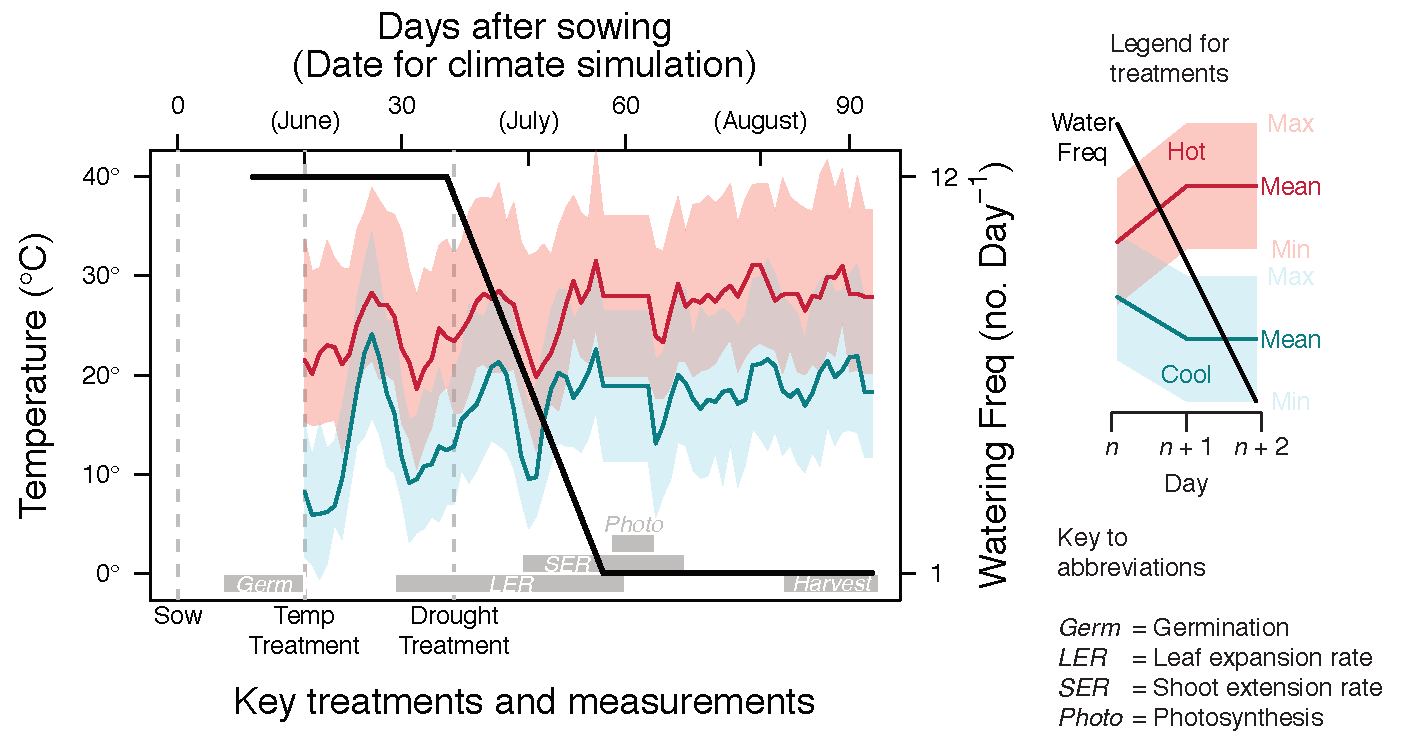
\includegraphics[width=1\textwidth]{Figures/Figure_ExptlDes.pdf}}
	\usefont{T1}{phv}{m}{n}
	\fontsize{10}{12}
	\selectfont
	\caption[Experimental Design]{Overview of experimental treatments and timing of key trait measurements. All plants germinated within 21 days of sowing. At that time, we began temperature treatments (left axis), simulating a typical June-August weather pattern at Hot (red) and Cold (blue) sites. The bold lines track the average daily temperatures. Within each day, there was a maximum daytime temperture (top of translucent polygons) and minimum nighttime temperature (bottom of translucent polygons). The drought treatment commenced later by ramping down the frequency of bottom-watering episodes (black line; right axis). Grey boxes on the bottom of the plot outline the period of key measurements described in the Methods.}
	\label{fig:Fig_ExptlDes}
\end{figure}

\subsection*{Growth and photosynthesis}

%%%%%%%%%%%%%%%%%%%%%%%%%%%%%%%%%%%%%%%%%%%%%%%%%%%%%%%%%%%%%%%%%%%%%%%%%%%%%%%%
% Table of key traits
%%%%%%%%%%%%%%%%%%%%%%%%%%%%%%%%%%%%%%%%%%%%%%%%%%%%%%%%%%%%%%%%%%%%%%%%%%%%%%%%

\begin{table}[ht]
   \centering
   \topcaption{Key traits measured in this study.}
   \begin{tabular}{@{} ll @{}}
      \toprule
  Trait & Units \\
      \midrule
  Day of germination  & day \\
  Leaf expansion rate  &  mm day$^{-1}$  \\
  Shoot elongation rate  &  mm or cm day$^{-1}$  \\
  Harvest dry mass &  g  \\
  Photosynthetic rate &  $\mu$mol CO$_2$ m$^{-2}$ s$^{-1}$\\
  Mortality &  \cdm{Probability?}  \\
	    \bottomrule
   \end{tabular}
   \label{table:Table_traits}
\end{table}

\paragraph{Day of germination} We tested for population variation in germination rate, measured as Days to Germination, using a lognormal survival model fit using the survreg function in the R package \pkg{survival} version 2.38 \citep{Therneau_2015}. The model was fit with Population as a fixed effect and Family as random effect using a $\Gamma$ frailty function. The signifcance of the Population effect was determined using analysis of deviance.


\paragraph{Growth rate: leaf expansion and shoot elongation}

We censused leaf length twice per week from 12 May -- 12 June (28--59 days after sowing), resulting in 10 measurements. We ceased measuring leaf length once it appeared to asymptote and growth shifted to shoot elongation.  We also censused plant height on 7 days (twice per week) between 29 May and 20 June (45 to 67 days after sowing). Both leaf expansion and shoot elongation were modeled as a second-order polynomials of time with individual coefficients (separate for leaf and shoot growth) using empirical Bayes' estimates from linear mixed-effects models fit using the R package \pkg{lme4} version 1.1-7 \citep{Bates_etal_2014}.




\paragraph{Photosynthesis}
During the week of 10 to 16 June (57 to 63 days after sowing), we measured daytime photosynthetic rate and stomatal conductance on a subset of 329 plants evenly spread between treatments and families within populations. The youngest, fully-expanded leaf \cdm{this is what I did...not sure exactly which node, as I didn't record that when I did measurements} acclimated for 3 minutes to reach steady state in a 6 cm$^2$ chamber of a LI-COR 6400XT Portable Photosynthesis System (LI-COR Biosciences, Lincoln, Nebraska). All measurements were made at ambient light (400 $\mu$mol m$^{-2}$ s$^{-1}$), temperature, and moderate relative humidity. During this period, we suspended normal day-to-day temperature fluctuations and set daytime temperatures to its average for that period (Cool: 26.5$\degree$; Hot: 36.1$\degree$ so that all plants within a temperature level were measured under the same conditions.


\paragraph{Mortality}
We assayed mortality during twice-weekly growth measurements. We could not get GLMM with Family effects to converge, so we used GLM with a quasibinomial error structure and assessed signifiance using Type 2 Analysis of Deviance with the R package \pkg{car}. 


\paragraph{Biomass at harvest} 

\cdm{show correlation between growth rate and biomass?}

\subsection*{Intrinsic variation and plasticity}

For all traits (Table~\ref{table:Table_traits}) we tested for Population, Treatment, and Population $\times$ Treatment interactions. We interpreted significant Population effects to indicate intrinsic variation and Population by Treatment effects to indicate variation in plasticity. As mentioned above, we survival and GLM models for germination rate and mortality, respectively. For all other traits, we used mixed model ANOVAs with Family included as a random factor. Models were fit by restricted maximum likelihood using lmer from the R package \pkg{lme4} \citep{Bates_etal_2014}. Significant fixed effect terms were selected using a step-wise backward elimination procedure implemented with the step function in the R package \pkg{lmerTest} version 2.0-11 \citep{Kuznetsova_etal_2014}. Denominator degrees of freedom for $F$-tests were estimated using Satterthwaite's approximation. Significant Population effect indicate intrinsic trait differences; significant Population $\times$ Treatment effects indicate population differences in plasticity. For growth rate, we also accounted for differences in germination rate by including day of germination as a factor.

\subsection*{Principal components of germination, growth, and photosynthesis}
For each single-trait model above, we extracted the Population coefficient (factoring out Treatment and other effects). The multivariate distribution of these coefficients was then summarized using principal components analysis (PCA). The first principal component of these traits (Trait PC1) loaded positively with germination, growth, and photostynthetic rate, therefore we define this as a phenotypic axis dilineating fast and slow growing populations.



\subsection*{Selective agents and environmental correlates}

We found that a population's position along PC1 correlated strongly with the latitude or origin (see Results). Since latitude \textit{per se} cannot be a selective agent, we considered three possible explanations. First, latitude may be strongly correlated, in this species, with one or two climatic variables, such as temperature, precipitation, or growing degree-days. Second, latitude may be correlated with several climatic agents of selection that are individually weak, but add up to a strong latiduinal cline. Third, gene flow among neighboring populations could smooth out local climatic effects, since alleles will experience selection across populations linked by migration. For example, average temperature of \textit{M. cardinalis} populations at a given latitude varies widely, but in aggregate, a Southern metapopulation experiences warmer climate than a Northern one. Thus, any particular Southern population would be warm-adapted, even if it was located in cooler (e.g. high elevation) site. 

To evaluate support for these hypotheses, we used Random Forest regression \citep{Liaw_Wiener_2002} to identify putative climatic factors underlying trait-latitude associations in \textit{M. cardinalis}. We looked for overlap between climatic variables that best predict latitude of \textit{M. cadinalis} occurence records and a separate analysis of climatic variables that best predict trait variation across our 16 focal populations. For brevity, we refer to these as Climate-Latitude and Climate-Trait variables. We selected Climate-Latitude and Climate-Trait variables independently using Random Forest (VSURF algorithm in the R \pkg{VSURF} version 0.8.2 \citep{Genuer_etal_2014}). From VSURF models, we kept only variables selected for prediction, the most stringent criterion.

The first hypothesis predicts that there should be one or two Climate-Latitude and Climate-Trait associations that are strongly correlated, whereas the second hypothesis predicts that several climatic variables should be weakly correlated. To test the third hypothesis about gene flow smoothing out local climatic variation, we repeated the same procedure to identify Climate-Trait variables as above, except that we used spatially averaged climate variables. We sampled climate at 1000 random points (at 90-m resolition) within a 100-km buffer around focal populations. We chose this buffer size because neutral genetic differentiation increases slowly with geographic distance, indicating significant gene flow between nearby populations \citep{Paul_etal_2016}. Since \textit{M. cardinalis} is found exclusively in riparian areas, we only selected points along streams using the National Hydrogeoraphy Dataset \citep{NHD}. Climatic means and CVs were weighted by their climatic suitability as determined using a multimodel ensemble average of ecological niche models \citep{Angert_ENM}. For clarity, we distinguish between analyses where climate is inferred from a single point (`point estimated Climate-Trait') versus averaged across a 100-km buffer (`spatially averaged Climate-Trait'). 

